\documentclass[10pt,a4paper]{article}
\usepackage[T1]{fontenc}
\usepackage{lmodern}
\usepackage{amssymb}
\usepackage[margin=2cm]{geometry}
\usepackage{graphicx}
\usepackage{booktabs}
\usepackage{float}
\usepackage{tabularx}
\usepackage{array}
\setlength{\parskip}{4pt}
\setlength{\parindent}{0pt}
\begin{document}
\begin{center}{\Large\bfseries Multivariable Constrained Optimisation of Aircraft Design for Maximum Flight Range}\\[4pt]
{\small AIT 203 Optimisation. Auto-generated by scripts/main\_report.py on 2026-11-26 20:18 from results/results.json. Do not edit by hand.}\end{center}
\section{Problem}
We choose the wing area S, aspect ratio AR, cruise speed V, fuel mass W\_fuel and initial cruise mass W\_i to maximise the jet Breguet range. Maximising R is the same as minimising f = $-$ln R, because ln is monotonic. The logarithm turns the product into a sum, which gives simpler gradients and makes every multiplier an elasticity (\% range per \% of a limit).

R = (V / c\_T) $\cdot$ (C\_L / C\_D) $\cdot$ ln(W\_i / (W\_i $-$ W\_fuel)),   C\_L = 2 W\_i g / ($\rho$ V\textsuperscript{2} S),   C\_D = C\_D0 + C\_L\textsuperscript{2} / ($\pi$ e AR)

\begin{table}[H]\centering\small
\begin{tabularx}{\textwidth}{l>{\raggedright\arraybackslash}X>{\raggedright\arraybackslash}X}
\toprule
\textbf{Constraint} & \textbf{Normalised form ($\le$ 0 unless = 0)} & \textbf{Meaning} \\
\midrule
weight build-up (= 0) & (W\_fixed + k\_w S\textasciicircum{}a AR\textasciicircum{}b W\_i\textasciicircum{}c + W\_fuel + W\_res + W\_pay) / W\_i $-$ 1 & the aircraft's mass adds up \\
MTOW & W\_i / MTOW $-$ 1 & not heavier than the maximum take-off mass \\
stall & (W\_i g / S) / ($\frac{1}{2}$ $\rho$$_0$ V\_stall\textsuperscript{2} C\_L,max) $-$ 1 & slow enough to land \\
fuel volume & (W\_fuel + W\_res) $\surd$AR / (k\_f S\textasciicircum{}1.5) $-$ 1 & fuel fits in the wing \\
Mach & V / (M\_max a) $-$ 1 & replaces a wave-drag model \\
gate span (separate case) & $\surd$(S$\cdot$AR) / b\_max $-$ 1 & fits a 36 m ICAO code C gate \\
bounds & x\_min $\le$ x $\le$ x\_max & keeps the search in a sensible box \\
\bottomrule
\end{tabularx}
\end{table}
\section{Parameters and where they come from}
Published values are Boeing 737-800 data. Calibrated values are fitted so that the model reproduces the 737-800 (Section 4). Assumed values are our choices and are listed with reasons in docs/assumptions.md.

\begin{table}[H]\centering\small
\begin{tabularx}{\textwidth}{l>{\raggedright\arraybackslash}X>{\raggedright\arraybackslash}X>{\raggedright\arraybackslash}X>{\raggedright\arraybackslash}X}
\toprule
\textbf{Parameter} & \textbf{Symbol} & \textbf{Value} & \textbf{Unit} & \textbf{Source} \\
\midrule
Maximum take-off mass & MTOW & 79,016 & kg & published (737-800) \\
Payload: 162 pax x 100 kg & W\_pay & 16,200 & kg & assumed (standard pax + bag mass) \\
Reserve fuel (carried, not burnt) & W\_res & 2,500 & kg & assumed \\
Zero-lift drag coefficient & CD0 & 0.02 & - & assumed (typical narrow-body) \\
Oswald efficiency & e & 0.8 & - & assumed (typical swept wing) \\
Max lift coefficient, landing flaps & CLmax & 2.6 & - & assumed (flapped narrow-body) \\
Maximum allowed stall speed & V\_stall\_max & 64 & m/s & assumed (737 baseline = 62.3 m/s fits) \\
Mach limit (replaces wave drag) & M\_max & 0.8 & - & assumed (between cruise 0.785 and MMO 0.82) \\
Cruise altitude & h\_cruise & 35,000 & ft & typical 737 cruise \\
Effective cruise TSFC & cT & 0.6999 & lb/(lbf h) & calibrated (literature 0.627) \\
Wing-mass exponent on S & a & 0.749 & - & Raymer eq. 15.25 (0.649 + 0.1 from S\_cs) \\
Wing-mass exponent on AR & b & 0.5 & - & Raymer eq. 15.25 \\
Wing-mass exponent on W\_i & c & 0.557 & - & Raymer eq. 15.25 \\
Wing-mass coefficient & k\_w & 0.09368 & - & calibrated (Raymer mass at 737 geometry) \\
Fixed mass (OEW minus wing) & W\_fixed & 35,722 & kg & calibrated (published OEW) \\
Fuel-volume coefficient & k\_f & 46.02 & kg/m\textasciicircum{}3 & calibrated (published tank capacity) \\
\bottomrule
\end{tabularx}
\end{table}
\section{Method}
\begin{itemize}\setlength{\itemsep}{1pt}
\item \textbf{Elimination of W\_fuel.} W\_fuel appears linearly in the weight build-up, so the custom solver computes it from (S, AR, V, W\_i). Every iterate is then a weight-consistent aircraft and the problem has 4 variables and inequality constraints only.
\item \textbf{Augmented Lagrangian (our own).} L\_A = f + (1/2$\mu$) $\Sigma$ [max(0, $\lambda$$_i$ + $\mu$ g$_i$)\textsuperscript{2} $-$ $\lambda$$_i$\textsuperscript{2}]. After each subproblem $\lambda$ $\leftarrow$ max(0, $\lambda$ + $\mu$ g), which keeps $\lambda$ $\ge$ 0. $\mu$ grows $\times$10 when the violation does not drop by a factor 4. A pure penalty method would need $\mu$ $\rightarrow$ $\infty$; the multiplier update keeps $\mu$ moderate and gives the KKT multipliers at the end.
\item \textbf{Inner solvers (our own).} Gradient descent, Newton, modified Newton (H + $\eta$I with $\eta$ = $\delta$ $-$ $\lambda$\_min when $\lambda$\_min $\le$ 0), BFGS and SR1, all with Armijo backtracking (c$_1$ = 10\textsuperscript{-}\textsuperscript{4}, halving). Newton-type methods use a central-difference Hessian of the analytic gradient.
\item \textbf{Reference solver.} SciPy SLSQP on the original 5-variable problem with the equality constraint. It checks both our solver and the W\_fuel elimination.
\item \textbf{Independent KKT check.} At the returned design, the multipliers are re-estimated by least squares on the active constraints, then stationarity, $\lambda$ $\ge$ 0 and complementarity are tested, and the Hessian of the Lagrangian is projected on the tangent space (second-order condition).
\item All variables are scaled to O(1) and all gradients are analytic (checked against finite differences in tests/).
\end{itemize}
\section{Calibration against the 737-800}
\begin{table}[H]\centering\small
\begin{tabular}{lr}
\toprule
\textbf{Item} & \textbf{Value} \\
\midrule
Published range (162 passengers) & 5,436 km (2935 nmi) \\
Raymer wing mass at 737-800 geometry & 5,691 kg, so W\_fixed = 35,722 kg \\
Fuel-volume coefficient k\_f & 46.02 kg/m\textsuperscript{3} \\
Range with literature TSFC 0.627 lb/lbf/h & 6,068 km (+11.6 \%) \\
Effective TSFC that reproduces the published range & 0.700 lb/lbf/h (used everywhere) \\
\bottomrule
\end{tabular}
\end{table}
Breguet cruise ignores taxi, take-off, climb and descent, so it over-predicts range by 11.6 \% with the literature TSFC. The effective TSFC absorbs these effects. Because c\_T only adds the constant ln c\_T to f, it changes the range level but \textbf{not the optimal design}. This is a consistency check, not an independent validation.

\section{Optimised design vs the 737-800}
\begin{table}[H]\centering\small
{\textbf{Range gain: +4.96 \% (no span limit), +4.21 \% (36 m span)}}\\[3pt]
\begin{tabularx}{\textwidth}{l>{\raggedright\arraybackslash}X>{\raggedright\arraybackslash}X>{\raggedright\arraybackslash}X}
\toprule
\textbf{} & \textbf{737-800 (model)} & \textbf{Optimum} & \textbf{Optimum, 36 m span} \\
\midrule
Range [km] & 5,436 & 5,705 & 5,665 \\
Wing area [m\textsuperscript{2}] & 124.6 & 132.4 & 128.3 \\
Aspect ratio & 9.45 & 11.77 & 10.10 \\
Span [m] & 34.32 & 39.48 & 36.00 \\
Cruise Mach & 0.785 & 0.800 & 0.800 \\
L/D & 17.07 & 18.18 & 17.34 \\
C\_L & 0.600 & 0.548 & 0.565 \\
Wing mass [kg] & 5,691 & 6,673 & 6,039 \\
Trip fuel [kg] & 18,316 & 17,921 & 18,555 \\
W\_i [kg] & 78,429 & 79,016 & 79,016 \\
Stall speed [m/s] & 62.3 & 60.6 & 61.6 \\
Active constraints & fuel volume & MTOW, fuel volume, Mach limit & MTOW, fuel volume, Mach limit, gate span \\
\bottomrule
\end{tabularx}
\end{table}
\begin{figure}[H]\centering
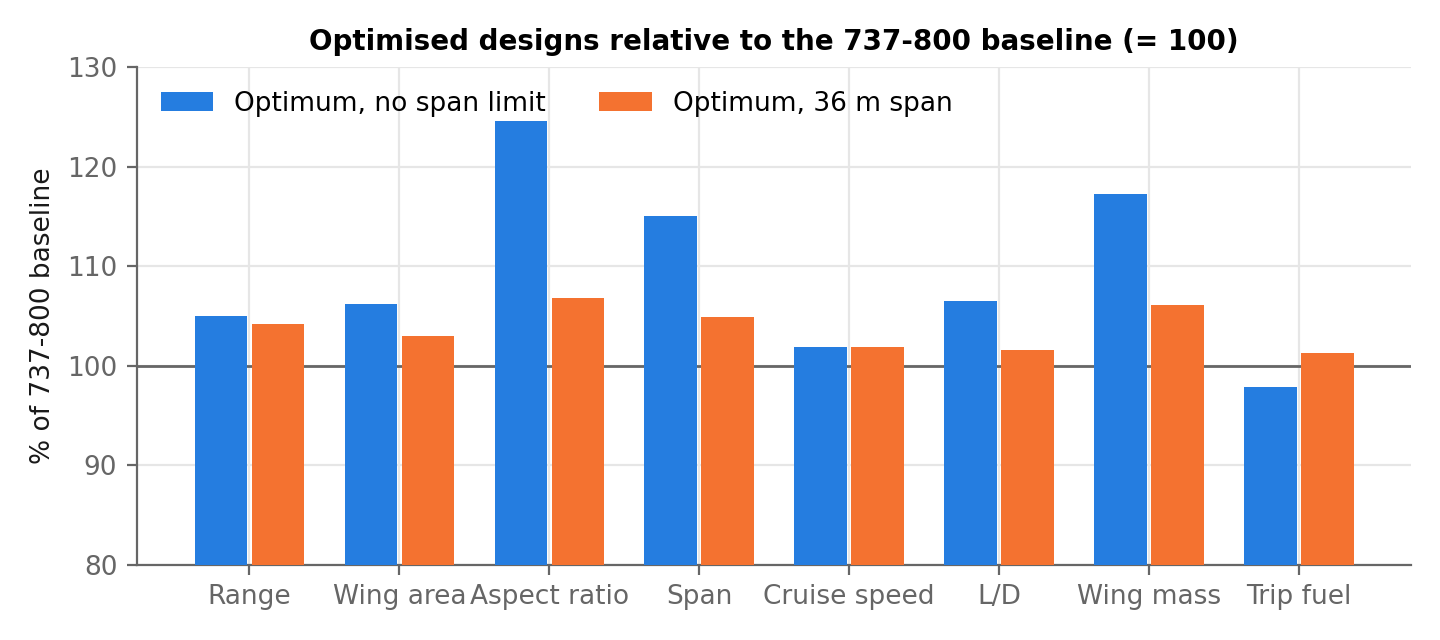
\includegraphics[width=0.9\textwidth]{figures/fig1_design_comparison.png}
\par\small\textit{Optimised designs relative to the 737-800 (= 100).}
\end{figure}
\begin{itemize}\setlength{\itemsep}{1pt}
\item The optimiser adds 982 kg of wing for a higher aspect ratio (AR 9.45 $\rightarrow$ 11.77). L/D rises by 6.5 \%, which outweighs the 2.2 \% less trip fuel.
\item Wing area grows just enough for the tanks to hold the fuel the MTOW allows, so MTOW and fuel volume are active together.
\item The speed goes to the Mach limit: range $\propto$ V$\cdot$L/D and without wave drag nothing penalises speed. This is a known artefact of replacing wave drag by a Mach cap.
\item AR stops short of its bounds: the heavier wing (AR\textasciicircum{}0.5) and the smaller tank (1/$\surd$AR) balance the lower induced drag.
\item The 36 m gate limit cuts the span from 39.5 m to 36.0 m. The wing area also shrinks (132.4 $\rightarrow$ 128.3 m\textsuperscript{2}), so AR = b\textsuperscript{2}/S only falls from 11.77 to 10.10. It costs 0.71 \% of the unrestricted optimum's range.
\item Our ALM and SLSQP agree to 1.8$\cdot$10\textsuperscript{-}\textsuperscript{8} (no span) and 2.0$\cdot$10\textsuperscript{-}\textsuperscript{8} (36 m) relative difference in x.
\end{itemize}
\section{Analysis}
\subsection{Payload-range}
\begin{figure}[H]\centering
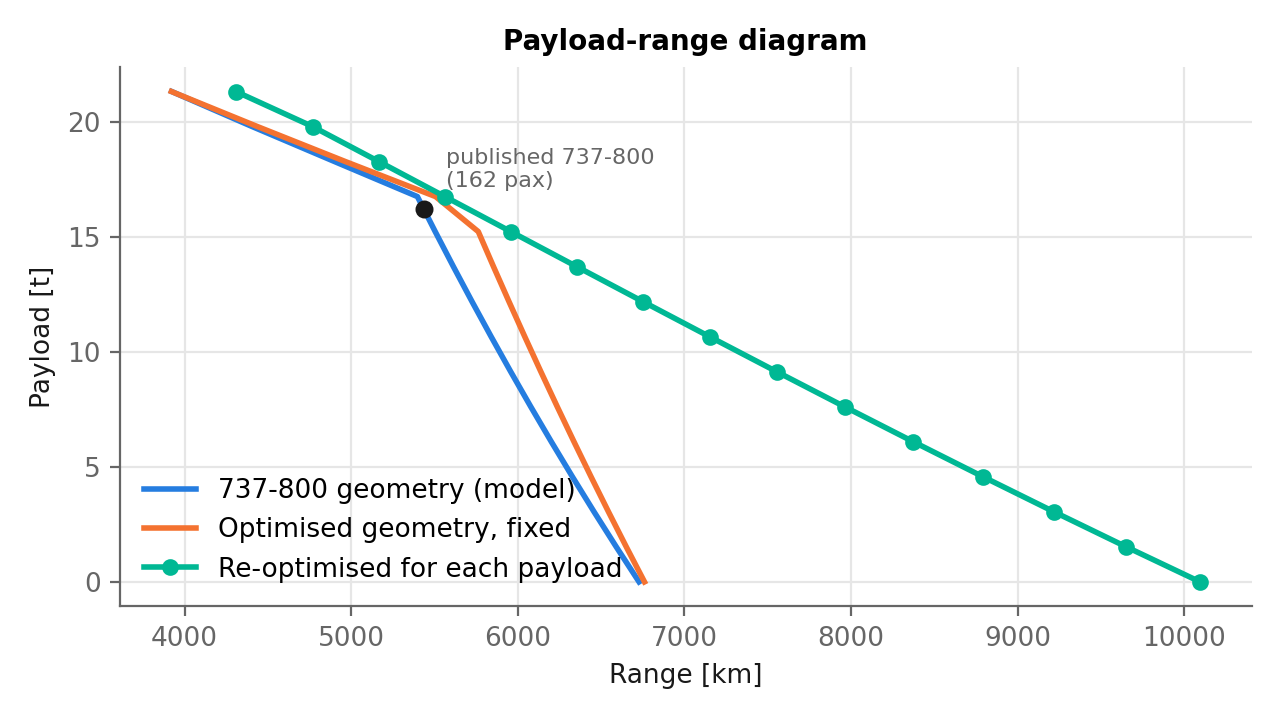
\includegraphics[width=0.9\textwidth]{figures/fig4_payload_range.png}
\par\small\textit{Payload-range diagram.}
\end{figure}
\begin{itemize}\setlength{\itemsep}{1pt}
\item \textbf{737-800 geometry}: the classic diagram, MTOW-limited at high payload and tank-limited at low payload. It passes through the published point by construction.
\item \textbf{Optimised geometry, fixed}: the nominal optimum flown at other payloads; up to 259 km more than the 737.
\item \textbf{Re-optimised for each payload}: at zero payload the best wing is S = 174 m\textsuperscript{2}, AR 8.4 (big tanks); at the 21.3 t structural maximum it is S = 119 m\textsuperscript{2}, AR 16.0 (active: MTOW, stall speed, Mach limit). The best wing depends strongly on the design mission.
\end{itemize}
\subsection{Lighter structures (k\_w)}
\begin{figure}[H]\centering
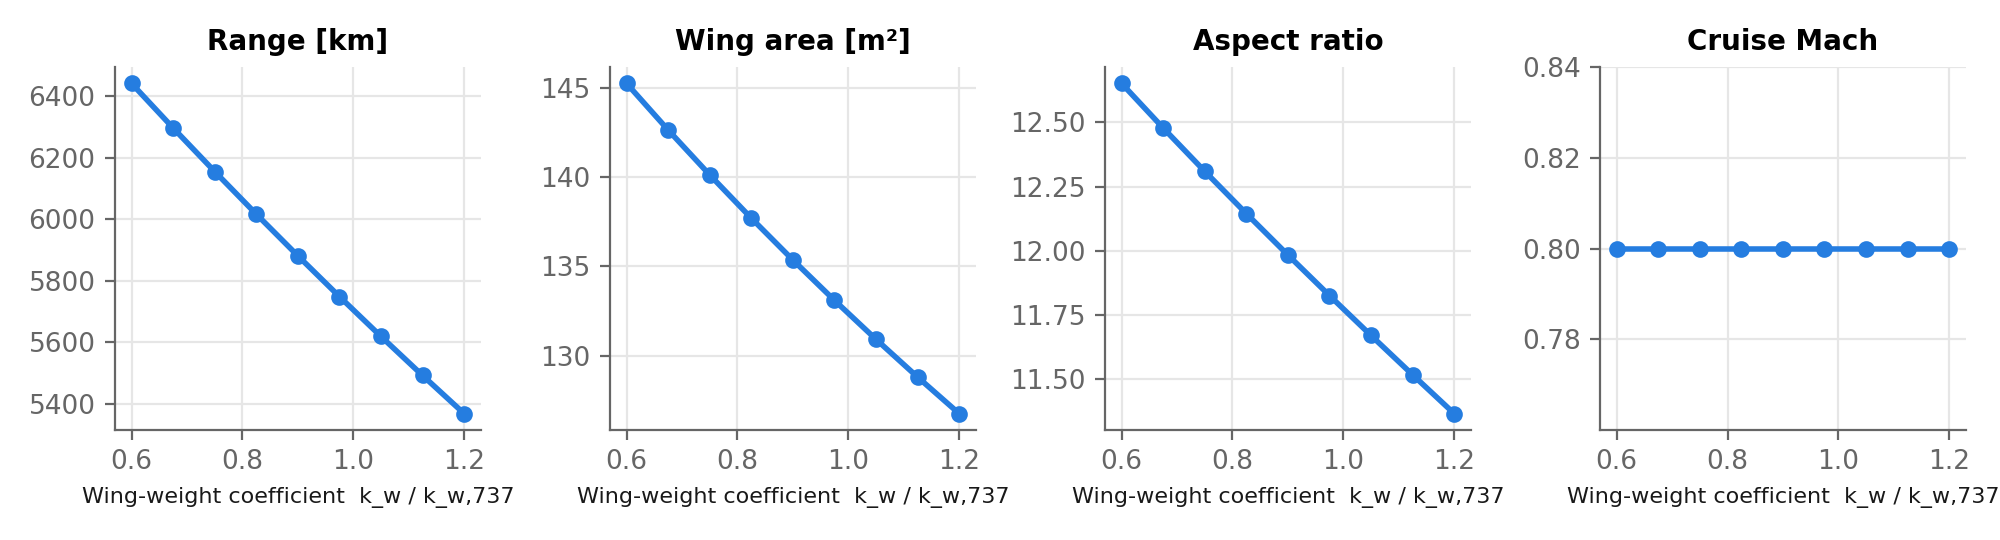
\includegraphics[width=0.9\textwidth]{figures/fig5_sweep_k_w.png}
\par\small\textit{Effect of the wing-weight coefficient.}
\end{figure}
Going from 1.20$\times$ to 0.60$\times$ the 737 wing-weight coefficient raises range from 5,368 to 6,441 km. The wing grows (S 127 $\rightarrow$ 145 m\textsuperscript{2}, AR 11.4 $\rightarrow$ 12.7) because lighter structure makes area and span cheaper.

\subsection{Stricter stall speed}
\begin{figure}[H]\centering
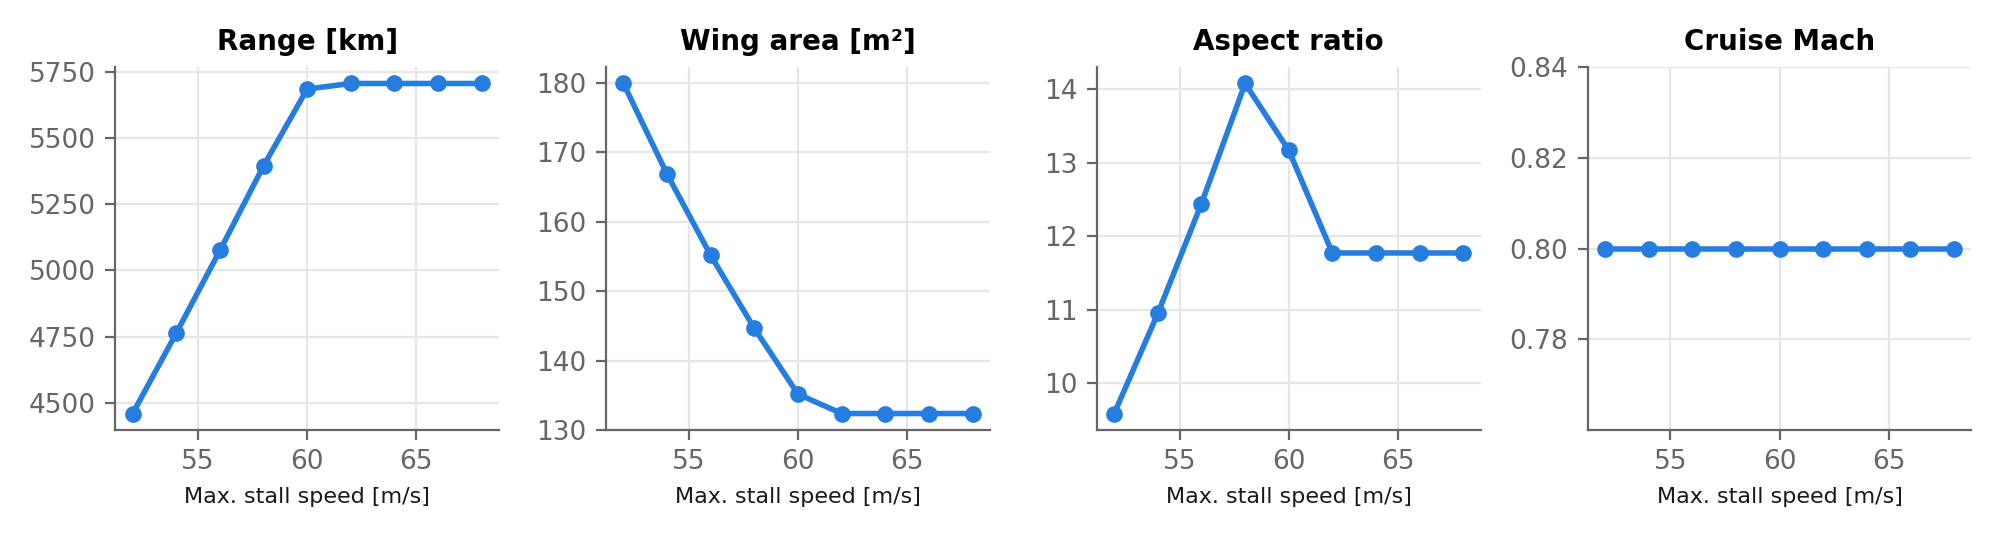
\includegraphics[width=0.9\textwidth]{figures/fig7_sweep_V_stall_max.png}
\par\small\textit{Effect of the maximum stall speed.}
\end{figure}
The stall limit is active for V\_stall,max $\le$ 60 m/s and inactive above. When active it forces a larger wing:

\begin{table}[H]\centering\small
\begin{tabular}{lrrrr}
\toprule
\textbf{V\_stall,max [m/s]} & \textbf{Wing area [m\textsuperscript{2}]} & \textbf{AR} & \textbf{Range [km]} & \textbf{vs unrestricted optimum} \\
\midrule
52 & 180 & 9.59 & 4,460 & -21.8 \% \\
54 & 167 & 10.95 & 4,764 & -16.5 \% \\
56 & 155 & 12.45 & 5,075 & -11.0 \% \\
58 & 145 & 14.08 & 5,395 & -5.4 \% \\
60 & 135 & 13.17 & 5,684 & -0.4 \% \\
\bottomrule
\end{tabular}
\end{table}
\subsection{More efficient engines (c\_T)}
\begin{figure}[H]\centering
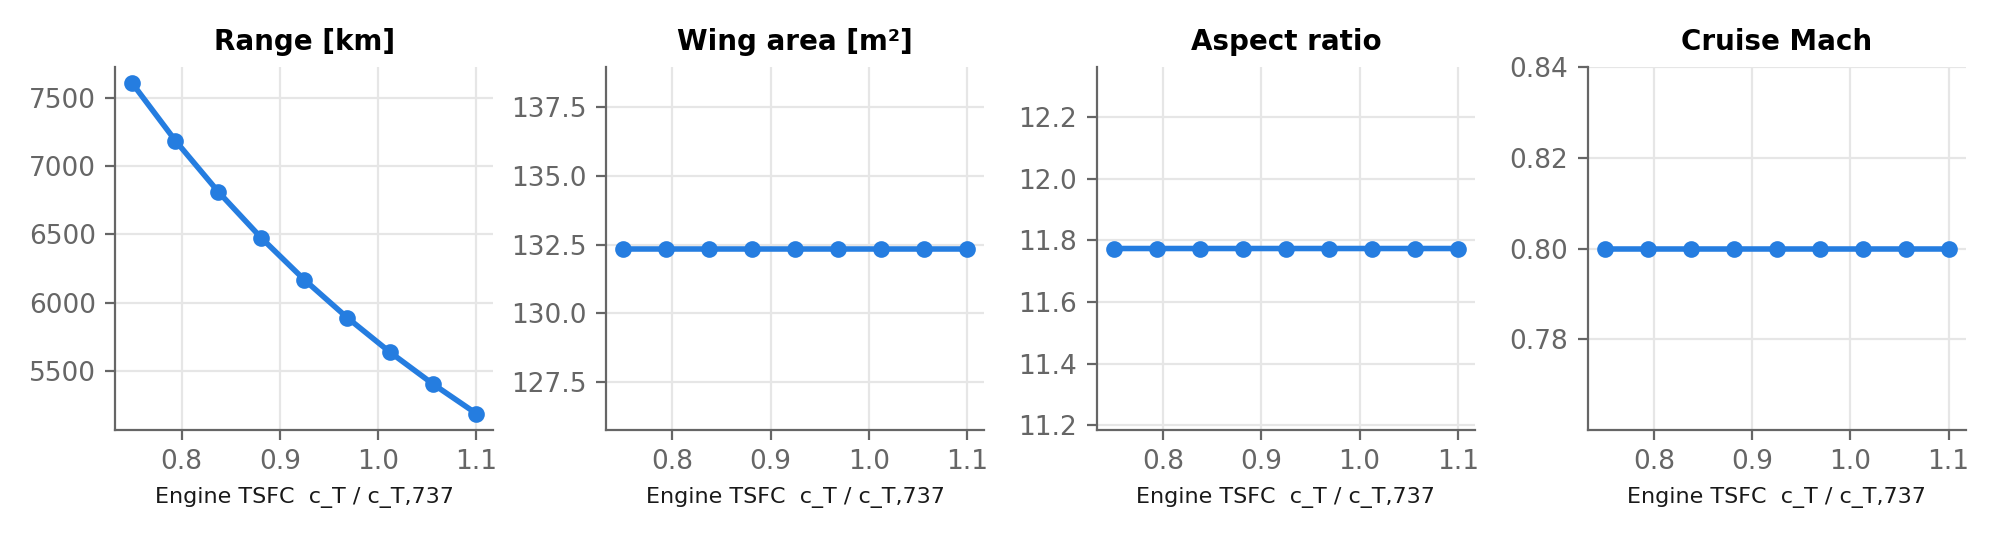
\includegraphics[width=0.9\textwidth]{figures/fig6_sweep_cT.png}
\par\small\textit{Effect of engine TSFC.}
\end{figure}
Range goes from 5,187 km at 1.10$\times$ to 7,607 km at 0.75$\times$ the TSFC. R $\times$ (c\_T/c\_T,737) stays constant to 2.1$\cdot$10\textsuperscript{-}\textsuperscript{1}\textsuperscript{0}, so R $\propto$ 1/c\_T exactly. The wing area changes by at most 5.5$\cdot$10\textsuperscript{-}\textsuperscript{9} (relative): as predicted, \textbf{the optimal design does not depend on c\_T}. In reality engine weight and size would couple engine and airframe.

\subsection{Cruise altitude}
\begin{figure}[H]\centering
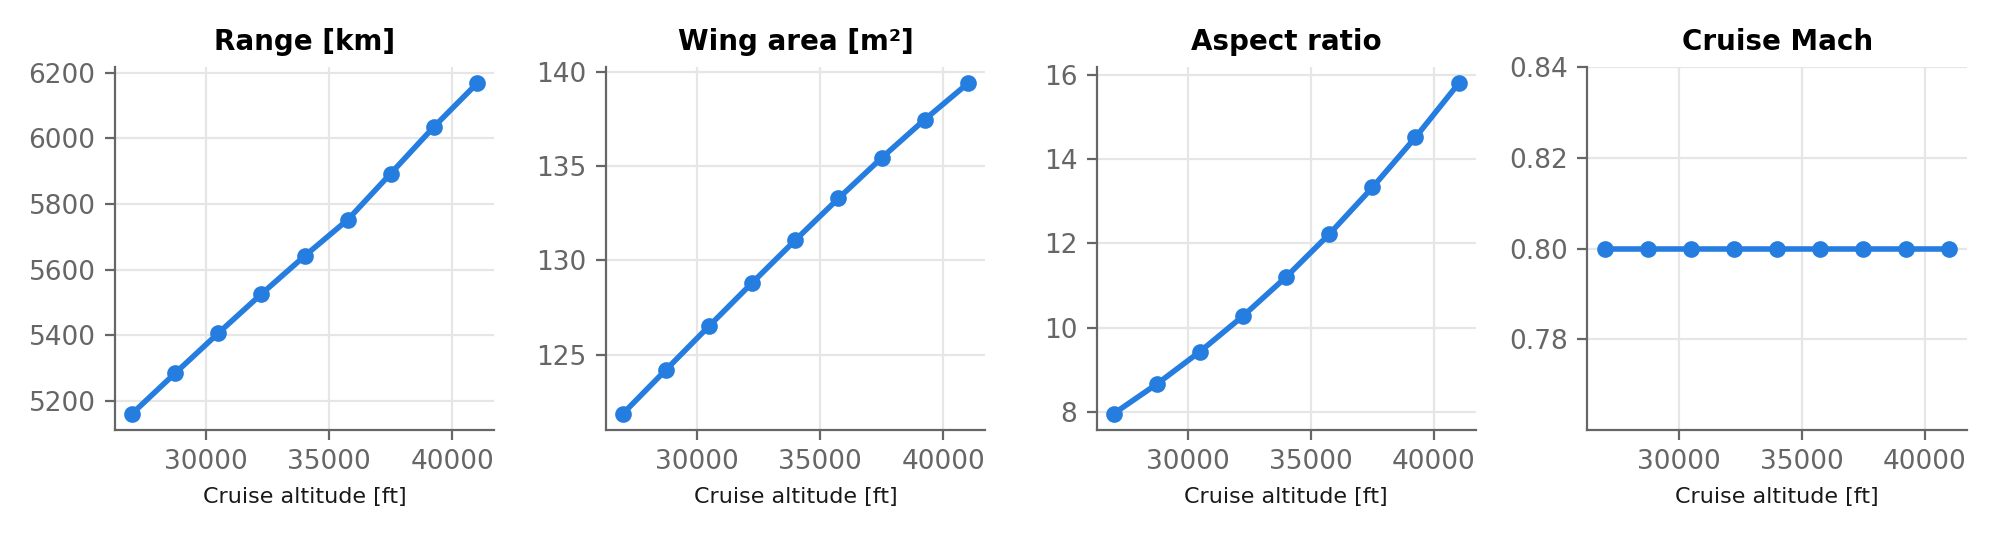
\includegraphics[width=0.9\textwidth]{figures/fig8_sweep_h_cruise.png}
\par\small\textit{Effect of cruise altitude.}
\end{figure}
From 27,000 ft to 41,000 ft range goes from 5,162 to 6,167 km and the optimal AR from 8.0 to 15.8: thinner air needs a higher C\_L, so induced drag matters more and span pays off. The model has no thrust lapse or buffet limit, so read this as 'what span is worth at a given altitude'.

\section{KKT conditions and multipliers as sensitivities}
\begin{table}[H]\centering\small
\begin{tabularx}{\textwidth}{l>{\raggedright\arraybackslash}X>{\raggedright\arraybackslash}X}
\toprule
\textbf{Check} & \textbf{No span limit} & \textbf{36 m span} \\
\midrule
Active & MTOW, fuel volume, Mach limit & MTOW, fuel volume, Mach limit, gate span \\
Stationarity residual & 3.4$\cdot$10\textsuperscript{-}\textsuperscript{1}\textsuperscript{0} & 6.7$\cdot$10\textsuperscript{-}\textsuperscript{1}\textsuperscript{6} \\
Smallest multiplier ($\ge$ 0 needed) & 0.347 & 0.156 \\
Complementarity & 1.2$\cdot$10\textsuperscript{-}\textsuperscript{8} & 1.2$\cdot$10\textsuperscript{-}\textsuperscript{8} \\
Second order & tangent space 1-dim, reduced Hessian eigenvalue(s) +0.403 & vertex: active gradients span R\textsuperscript{5} with positive multipliers \\
\bottomrule
\end{tabularx}
\end{table}
Both optima are strict local minima: yes. Because f = $-$ln R and every constraint is normalised, a multiplier $\lambda$$_i$ is the \% range gained per 1 \% relaxation of constraint i. By the envelope theorem dR/dp = $-$R $\partial$L/$\partial$p. Each prediction was checked by re-solving with the parameter increased by 1 \%:

\begin{table}[H]\centering\small
{\textbf{Sensitivities, no span limit}}\\[3pt]
\begin{tabular}{lrrr}
\toprule
\textbf{Parameter} & \textbf{dR/dp from KKT} & \textbf{Predicted $\Delta$R (+1 \%)} & \textbf{Re-solved $\Delta$R} \\
\midrule
MTOW & 0.1888 km per kg & +149.2 km & +148.0 km \\
M\_max & 2473 km per unit of Mach & +19.8 km & +19.4 km \\
k\_f & 45.81 km per kg/m\textsuperscript{3} of k\_f & +21.1 km & +21.0 km \\
W\_pay & -0.2598 km per kg & -42.1 km & -42.1 km \\
V\_stall\_max & 0 km per m/s & +0.0 km & +0.0 km \\
\bottomrule
\end{tabular}
\end{table}
\begin{table}[H]\centering\small
{\textbf{Sensitivities, 36 m span}}\\[3pt]
\begin{tabular}{lrrr}
\toprule
\textbf{Parameter} & \textbf{dR/dp from KKT} & \textbf{Predicted $\Delta$R (+1 \%)} & \textbf{Re-solved $\Delta$R} \\
\midrule
MTOW & 0.1814 km per kg & +143.3 km & +141.9 km \\
M\_max & 3860 km per unit of Mach & +30.9 km & +29.7 km \\
k\_f & 41.99 km per kg/m\textsuperscript{3} of k\_f & +19.3 km & +19.2 km \\
W\_pay & -0.2583 km per kg & -41.8 km & -41.8 km \\
V\_stall\_max & 0 km per m/s & +0.0 km & +0.0 km \\
b\_max & 24.57 km per m & +8.8 km & +8.3 km \\
\bottomrule
\end{tabular}
\end{table}
MTOW is the most valuable limit to relax: one extra tonne is worth about 189 km. The small gaps between prediction and re-solve are the second-order effects of a 1 \% step.

\section{Solver comparison}
ALM outer loop with each inner method, started from the 737-800 baseline.

\begin{table}[H]\centering\small
{\textbf{Solver comparison, no span limit}}\\[3pt]
\begin{tabularx}{\textwidth}{l>{\raggedright\arraybackslash}X>{\raggedright\arraybackslash}X>{\raggedright\arraybackslash}X>{\raggedright\arraybackslash}X>{\raggedright\arraybackslash}X>{\raggedright\arraybackslash}X>{\raggedright\arraybackslash}X>{\raggedright\arraybackslash}X}
\toprule
\textbf{Method} & \textbf{Conv.} & \textbf{Outer it.} & \textbf{Inner it.} & \textbf{$\nabla$f evals} & \textbf{Fallbacks} & \textbf{Capped subprobl.} & \textbf{Time [s]} & \textbf{Error vs SLSQP} \\
\midrule
Gradient descent & yes & 10 & 24,399 & 24,409 & 0 & 8 & 29.821 & 1.1$\cdot$10\textsuperscript{-}\textsuperscript{6} \\
Newton (FD Hessian) & yes & 9 & 24 & 225 & 2 & 0 & 0.032 & 1.8$\cdot$10\textsuperscript{-}\textsuperscript{8} \\
Modified Newton & yes & 9 & 24 & 225 & 0 & 0 & 0.039 & 1.8$\cdot$10\textsuperscript{-}\textsuperscript{8} \\
BFGS (default) & yes & 9 & 219 & 228 & 0 & 0 & 0.082 & 1.8$\cdot$10\textsuperscript{-}\textsuperscript{8} \\
SR1 & yes & 9 & 115 & 124 & 7 & 0 & 0.023 & 1.8$\cdot$10\textsuperscript{-}\textsuperscript{8} \\
SLSQP (SciPy, reference) & yes & 7 & - & 7 & 0 & 0 & 0.002 & 0 \\
\bottomrule
\end{tabularx}
\end{table}
\begin{table}[H]\centering\small
{\textbf{Solver comparison, 36 m span}}\\[3pt]
\begin{tabularx}{\textwidth}{l>{\raggedright\arraybackslash}X>{\raggedright\arraybackslash}X>{\raggedright\arraybackslash}X>{\raggedright\arraybackslash}X>{\raggedright\arraybackslash}X>{\raggedright\arraybackslash}X>{\raggedright\arraybackslash}X>{\raggedright\arraybackslash}X}
\toprule
\textbf{Method} & \textbf{Conv.} & \textbf{Outer it.} & \textbf{Inner it.} & \textbf{$\nabla$f evals} & \textbf{Fallbacks} & \textbf{Capped subprobl.} & \textbf{Time [s]} & \textbf{Error vs SLSQP} \\
\midrule
Gradient descent & yes & 9 & 11,444 & 11,453 & 0 & 3 & 21.140 & 2.6$\cdot$10\textsuperscript{-}\textsuperscript{8} \\
Newton (FD Hessian) & yes & 9 & 22 & 207 & 1 & 0 & 0.029 & 2.0$\cdot$10\textsuperscript{-}\textsuperscript{8} \\
Modified Newton & yes & 9 & 22 & 207 & 0 & 0 & 0.029 & 2.0$\cdot$10\textsuperscript{-}\textsuperscript{8} \\
BFGS (default) & yes & 9 & 184 & 193 & 0 & 0 & 0.058 & 2.0$\cdot$10\textsuperscript{-}\textsuperscript{8} \\
SR1 & yes & 9 & 125 & 134 & 13 & 0 & 0.050 & 2.0$\cdot$10\textsuperscript{-}\textsuperscript{8} \\
SLSQP (SciPy, reference) & yes & 4 & - & 4 & 0 & 0 & 0.001 & 0 \\
\bottomrule
\end{tabularx}
\end{table}
\begin{figure}[H]\centering
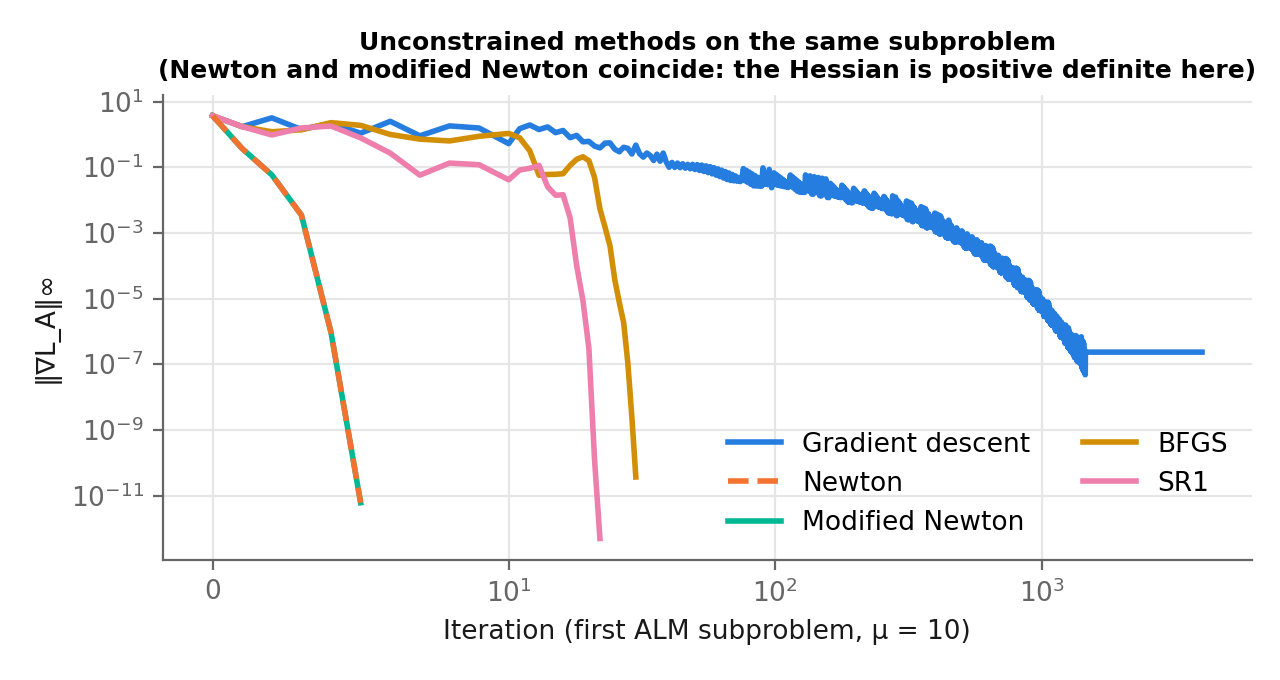
\includegraphics[width=0.9\textwidth]{figures/fig2_inner_convergence.png}
\par\small\textit{Inner methods on the same first ALM subproblem.}
\end{figure}
\begin{figure}[H]\centering
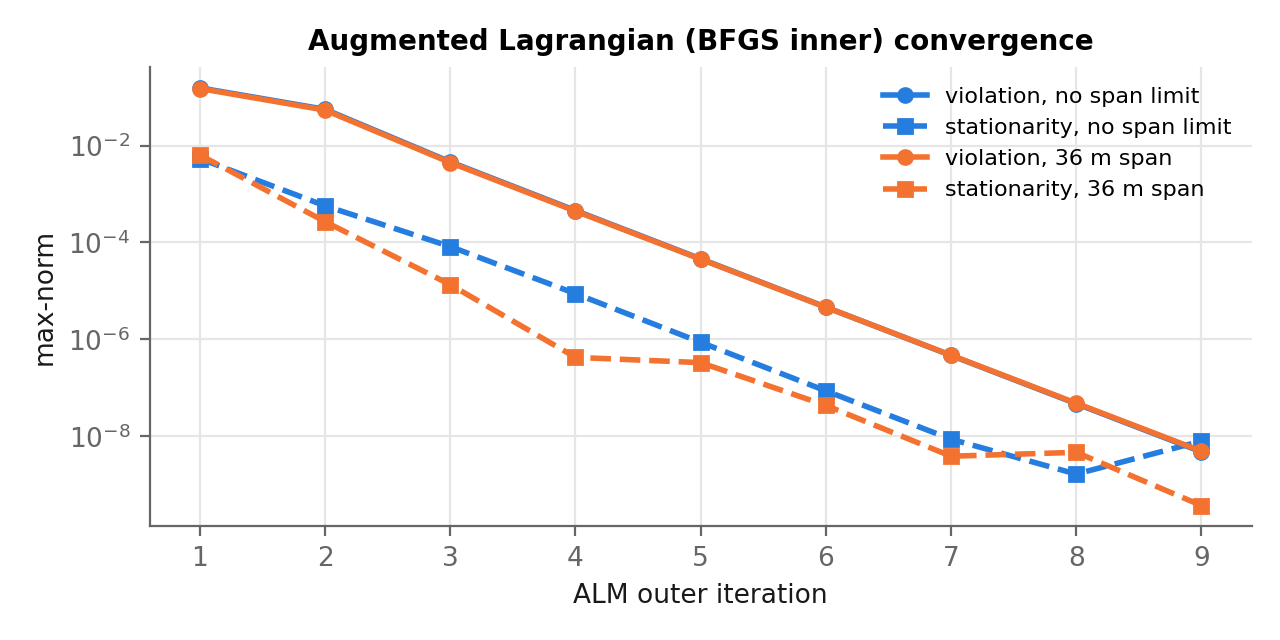
\includegraphics[width=0.9\textwidth]{figures/fig3_alm_convergence.png}
\par\small\textit{ALM outer convergence (BFGS inner solver).}
\end{figure}
\begin{itemize}\setlength{\itemsep}{1pt}
\item \textbf{Gradient descent} needs 24,399 inner iterations and hits the iteration cap in 8 subproblem(s). Growing $\mu$ makes L\_A ill-conditioned (the term $\mu$$\nabla$g$\nabla$g$^T$) and steepest descent zig-zags; it converges only linearly.
\item Without the span limit, \textbf{Newton} takes 24 inner iterations with 2 fallback(s) to $-$$\nabla$f, where the Hessian was not positive definite; \textbf{modified Newton} takes 24 with 0 fallbacks, because the eigenvalue shift always gives a descent direction.
\item With the span limit, \textbf{Newton} takes 22 inner iterations with 1 fallback(s) to $-$$\nabla$f, where the Hessian was not positive definite; \textbf{modified Newton} takes 22 with 0 fallbacks, because the eigenvalue shift always gives a descent direction.
\item \textbf{BFGS} (219 iterations, 0 resets) and \textbf{SR1} (115 iterations, 7 resets) need only gradients. SR1's matrix is not guaranteed positive definite, so it sometimes gives a non-descent direction and we reset it; BFGS keeps it positive definite whenever s$^T$y > 0.
\item \textbf{SLSQP} is fastest in wall time: it is compiled code and solves the 5-variable problem directly.
\end{itemize}
\section{Multi-start}
\begin{figure}[H]\centering
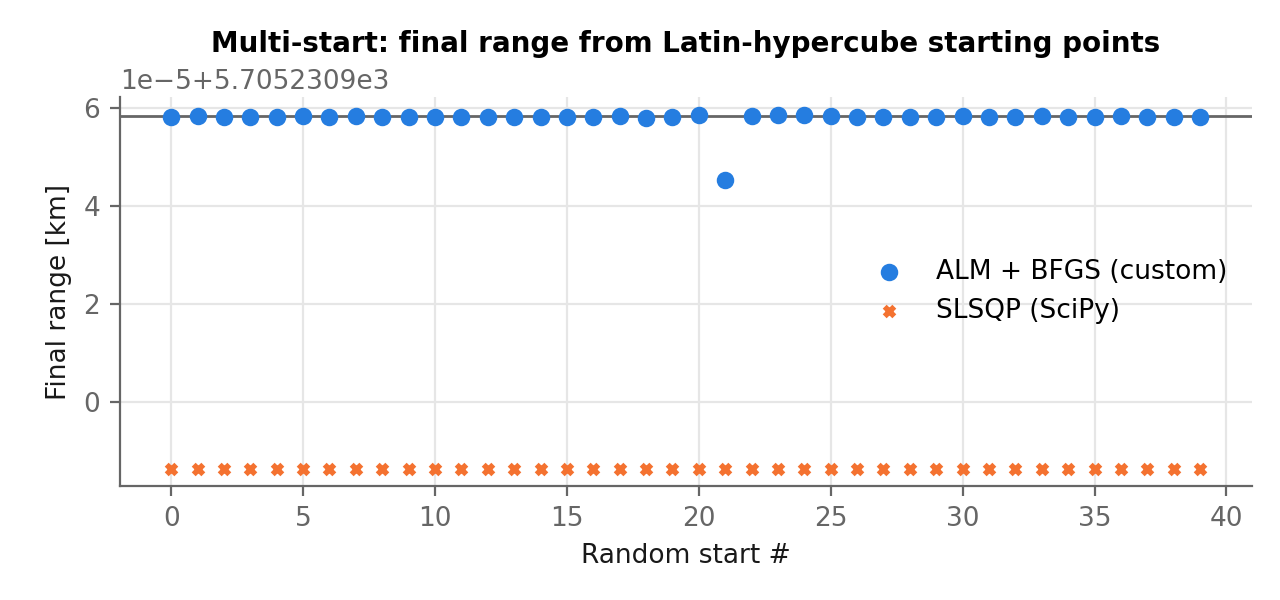
\includegraphics[width=0.9\textwidth]{figures/fig9_multistart.png}
\par\small\textit{Final range from Latin-hypercube starting points.}
\end{figure}
40 Latin-hypercube starting points over the whole box: ALM converged in 40, SLSQP succeeded in 40. Distinct final ranges (0.1 km rounding): 5,705.2 km. This is numerical evidence, not proof, that the optimum is global within the bounds (the problem is non-convex).

\section{Convergence audit}
All 51 optimisations inside the payload-range and sweep studies converged, and each agrees with SLSQP to better than 10\textsuperscript{-}\textsuperscript{5} (relative, in x).

\section{Limitations}
\begin{itemize}\setlength{\itemsep}{1pt}
\item No wave drag, so the Mach limit is always active and sets the speed.
\item Fixed altitude per run, no thrust or buffet limit; constant L/D and c\_T in cruise (Breguet).
\item No engine weight or size model, so engine and airframe decouple.
\item One cruise segment; climb, descent and step climbs are absorbed into the calibrated c\_T.
\item Wing mass and fuel volume are empirical scalings around the 737; designs far from it (AR > 14, S > 170 m\textsuperscript{2}) are extrapolations. Wing mass is not a strength model.
\item The stall constraint uses W\_i rather than landing weight (conservative), as in the proposal.
\item Results are model-predicted and calibrated on one aircraft; they are not a validated redesign.
\end{itemize}
\section{Reproducibility}
\texttt{pip install -r requirements.txt}, \texttt{python -m pytest}, \texttt{python scripts/run\_all.py}. This run: 98 s, Python 3.13.12, NumPy 2.3.2, SciPy 1.16.3, Matplotlib 3.10.8. Every table is also in results/tables/ as CSV.

\section{Appendix: full tables}
\begin{table}[H]\centering\small
{\textbf{Payload-range}}\\[3pt]
\begin{tabularx}{\textwidth}{l>{\raggedright\arraybackslash}X>{\raggedright\arraybackslash}X>{\raggedright\arraybackslash}X>{\raggedright\arraybackslash}X>{\raggedright\arraybackslash}X>{\raggedright\arraybackslash}X}
\toprule
\textbf{Payload [kg]} & \textbf{737 geometry [km]} & \textbf{Optimised, fixed [km]} & \textbf{Re-optimised [km]} & \textbf{Re-opt. S} & \textbf{Re-opt. AR} & \textbf{Active (re-opt.)} \\
\midrule
0 & 6,728 & 6,760 & 10,095 & 174.0 & 8.43 & MTOW, fuel volume, Mach limit \\
1,523 & 6,591 & 6,651 & 9,652 & 170.7 & 8.67 & MTOW, fuel volume, Mach limit \\
3,046 & 6,458 & 6,544 & 9,218 & 167.3 & 8.93 & MTOW, fuel volume, Mach limit \\
4,568 & 6,328 & 6,440 & 8,793 & 163.8 & 9.19 & MTOW, fuel volume, Mach limit \\
6,091 & 6,201 & 6,337 & 8,374 & 160.1 & 9.47 & MTOW, fuel volume, Mach limit \\
7,614 & 6,078 & 6,237 & 7,962 & 156.4 & 9.77 & MTOW, fuel volume, Mach limit \\
9,137 & 5,957 & 6,138 & 7,554 & 152.5 & 10.08 & MTOW, fuel volume, Mach limit \\
10,660 & 5,840 & 6,042 & 7,151 & 148.5 & 10.41 & MTOW, fuel volume, Mach limit \\
12,182 & 5,725 & 5,947 & 6,751 & 144.3 & 10.76 & MTOW, fuel volume, Mach limit \\
13,705 & 5,613 & 5,854 & 6,354 & 139.9 & 11.13 & MTOW, fuel volume, Mach limit \\
15,228 & 5,504 & 5,763 & 5,958 & 135.4 & 11.52 & MTOW, fuel volume, Mach limit \\
16,751 & 5,397 & 5,506 & 5,562 & 130.6 & 11.92 & MTOW, fuel volume, Mach limit \\
18,273 & 4,900 & 4,965 & 5,166 & 125.7 & 12.35 & MTOW, fuel volume, Mach limit \\
19,796 & 4,405 & 4,437 & 4,768 & 120.5 & 12.80 & MTOW, fuel volume, Mach limit \\
21,319 & 3,922 & 3,921 & 4,307 & 118.8 & 15.97 & MTOW, stall speed, Mach limit \\
\bottomrule
\end{tabularx}
\end{table}
\begin{table}[H]\centering\small
{\textbf{Sweep: Wing-weight coefficient  k\_w / k\_w,737}}\\[3pt]
\begin{tabular}{lrrrrrrr}
\toprule
\textbf{Value} & \textbf{Range [km]} & \textbf{S [m\textsuperscript{2}]} & \textbf{AR} & \textbf{Span [m]} & \textbf{Mach} & \textbf{L/D} & \textbf{Active} \\
\midrule
0.6 & 6,441 & 145.2 & 12.65 & 42.87 & 0.800 & 17.94 & MTOW, fuel volume, Mach limit \\
0.675 & 6,297 & 142.6 & 12.48 & 42.19 & 0.800 & 18.00 & MTOW, fuel volume, Mach limit \\
0.75 & 6,155 & 140.1 & 12.31 & 41.53 & 0.800 & 18.06 & MTOW, fuel volume, Mach limit \\
0.825 & 6,017 & 137.7 & 12.14 & 40.89 & 0.800 & 18.11 & MTOW, fuel volume, Mach limit \\
0.9 & 5,881 & 135.4 & 11.98 & 40.27 & 0.800 & 18.15 & MTOW, fuel volume, Mach limit \\
0.975 & 5,749 & 133.1 & 11.83 & 39.67 & 0.800 & 18.17 & MTOW, fuel volume, Mach limit \\
1.05 & 5,619 & 130.9 & 11.67 & 39.09 & 0.800 & 18.19 & MTOW, fuel volume, Mach limit \\
1.125 & 5,492 & 128.8 & 11.52 & 38.52 & 0.800 & 18.19 & MTOW, fuel volume, Mach limit \\
1.2 & 5,368 & 126.8 & 11.37 & 37.96 & 0.800 & 18.19 & MTOW, fuel volume, Mach limit \\
\bottomrule
\end{tabular}
\end{table}
\begin{table}[H]\centering\small
{\textbf{Sweep: Engine TSFC  c\_T / c\_T,737}}\\[3pt]
\begin{tabular}{lrrrrrrr}
\toprule
\textbf{Value} & \textbf{Range [km]} & \textbf{S [m\textsuperscript{2}]} & \textbf{AR} & \textbf{Span [m]} & \textbf{Mach} & \textbf{L/D} & \textbf{Active} \\
\midrule
0.75 & 7,607 & 132.4 & 11.77 & 39.48 & 0.800 & 18.18 & MTOW, fuel volume, Mach limit \\
0.7937 & 7,188 & 132.4 & 11.77 & 39.48 & 0.800 & 18.18 & MTOW, fuel volume, Mach limit \\
0.8375 & 6,812 & 132.4 & 11.77 & 39.48 & 0.800 & 18.18 & MTOW, fuel volume, Mach limit \\
0.8813 & 6,474 & 132.4 & 11.77 & 39.48 & 0.800 & 18.18 & MTOW, fuel volume, Mach limit \\
0.925 & 6,168 & 132.4 & 11.77 & 39.48 & 0.800 & 18.18 & MTOW, fuel volume, Mach limit \\
0.9688 & 5,889 & 132.4 & 11.77 & 39.48 & 0.800 & 18.18 & MTOW, fuel volume, Mach limit \\
1.013 & 5,635 & 132.4 & 11.77 & 39.48 & 0.800 & 18.18 & MTOW, fuel volume, Mach limit \\
1.056 & 5,401 & 132.4 & 11.77 & 39.48 & 0.800 & 18.18 & MTOW, fuel volume, Mach limit \\
1.1 & 5,187 & 132.4 & 11.77 & 39.48 & 0.800 & 18.18 & MTOW, fuel volume, Mach limit \\
\bottomrule
\end{tabular}
\end{table}
\begin{table}[H]\centering\small
{\textbf{Sweep: Max. stall speed [m/s]}}\\[3pt]
\begin{tabularx}{\textwidth}{l>{\raggedright\arraybackslash}X>{\raggedright\arraybackslash}X>{\raggedright\arraybackslash}X>{\raggedright\arraybackslash}X>{\raggedright\arraybackslash}X>{\raggedright\arraybackslash}X>{\raggedright\arraybackslash}X}
\toprule
\textbf{Value} & \textbf{Range [km]} & \textbf{S [m\textsuperscript{2}]} & \textbf{AR} & \textbf{Span [m]} & \textbf{Mach} & \textbf{L/D} & \textbf{Active} \\
\midrule
52 & 4,460 & 179.9 & 9.59 & 41.54 & 0.800 & 15.08 & MTOW, stall speed, Mach limit \\
54 & 4,764 & 166.9 & 10.95 & 42.75 & 0.800 & 16.18 & MTOW, stall speed, Mach limit \\
56 & 5,075 & 155.2 & 12.45 & 43.94 & 0.800 & 17.32 & MTOW, stall speed, Mach limit \\
58 & 5,395 & 144.6 & 14.08 & 45.13 & 0.800 & 18.50 & MTOW, stall speed, Mach limit \\
60 & 5,684 & 135.2 & 13.17 & 42.19 & 0.800 & 18.70 & MTOW, stall speed, fuel volume, Mach limit \\
62 & 5,705 & 132.4 & 11.77 & 39.48 & 0.800 & 18.18 & MTOW, fuel volume, Mach limit \\
64 & 5,705 & 132.4 & 11.77 & 39.48 & 0.800 & 18.18 & MTOW, fuel volume, Mach limit \\
66 & 5,705 & 132.4 & 11.77 & 39.48 & 0.800 & 18.18 & MTOW, fuel volume, Mach limit \\
68 & 5,705 & 132.4 & 11.77 & 39.48 & 0.800 & 18.18 & MTOW, fuel volume, Mach limit \\
\bottomrule
\end{tabularx}
\end{table}
\begin{table}[H]\centering\small
{\textbf{Sweep: Cruise altitude [ft]}}\\[3pt]
\begin{tabular}{lrrrrrrr}
\toprule
\textbf{Value} & \textbf{Range [km]} & \textbf{S [m\textsuperscript{2}]} & \textbf{AR} & \textbf{Span [m]} & \textbf{Mach} & \textbf{L/D} & \textbf{Active} \\
\midrule
2.7e+04 & 5,162 & 121.9 & 7.96 & 31.15 & 0.800 & 14.47 & MTOW, fuel volume, Mach limit \\
2.875e+04 & 5,285 & 124.2 & 8.67 & 32.81 & 0.800 & 15.20 & MTOW, fuel volume, Mach limit \\
3.05e+04 & 5,407 & 126.5 & 9.44 & 34.55 & 0.800 & 15.97 & MTOW, fuel volume, Mach limit \\
3.225e+04 & 5,526 & 128.8 & 10.28 & 36.39 & 0.800 & 16.79 & MTOW, fuel volume, Mach limit \\
3.4e+04 & 5,641 & 131.1 & 11.21 & 38.33 & 0.800 & 17.66 & MTOW, fuel volume, Mach limit \\
3.575e+04 & 5,752 & 133.3 & 12.22 & 40.36 & 0.800 & 18.58 & MTOW, fuel volume, Mach limit \\
3.75e+04 & 5,893 & 135.4 & 13.33 & 42.48 & 0.800 & 19.55 & MTOW, fuel volume, Mach limit \\
3.925e+04 & 6,035 & 137.5 & 14.52 & 44.67 & 0.800 & 20.56 & MTOW, fuel volume, Mach limit \\
4.1e+04 & 6,167 & 139.4 & 15.79 & 46.92 & 0.800 & 21.60 & MTOW, fuel volume, Mach limit \\
\bottomrule
\end{tabular}
\end{table}
\end{document}